
We deal here with the problem of augmenting visual information about an object
with motor information about it, that is the way the object can be grasped by
a human being. This can be seen as an instance of a more general framework for
multi-modal learning. Although a formal, abstract definition of this framework
is out of scope here, we outline it in order to clearly frame the point of view
from which we hope to improve classical object modelling and recognition.

In everyday life, living beings use \emph{distal} sensory modalities as their only
means of ``on-line'' gathering information about the world (by distal here we
mean, senses which operate at long distance such as, e.g., vision, hearing,
smell, etc.). This is coherent with the basic needs of avoiding predators,
finding food, mating and so on. Of course, (distal) sensorial information is
multi-modal in nature, as, e.g., the smell, sight and noise characteristic of a
predator come together in experience. But to our end, a more subtle form of multi-modal
learning is considered, that is, associating distal and \emph{proximal} modalities
in the infanthood, where by proximal we mean sensorimotor and proprioceptive: those
modalities which appeal to manipulation. Following Gibson's idea, for example,
the sight of an object would be inextricably associated by a human being to the
ways it can be used. This
association is primed by manipulation in the early development: at first randomly,
then in a more and more refined way. According to this, human object recognition
is so good also because we can reconstruct motor information associated to visual
information, and use it too when dealing with a new object.

With the goal of applying this idea to automated object recognition, we propose to build an object classification system 
on a set of visual {\em and} motor features. Whenever the motor features are not perceived by the system (i.e. the
agent is not grasping the object in the field of view), we infer them from the visual input through 
a mapping function, learned during training. This scheme mimics the early-development training mentioned above.
We now proceed to illustrate in detail our framework, that is summarized schematically in Figure \ref{fig:framework}.
We first describe the learning processes that occur during training, and then we describe the object classification
procedure during testing.

\vspace{0.5cm}
\noindent
{\bf Training} Figure \ref{fig:framework}, left, illustrates the learning processes activated during training. The system receives
as input visual and motor data. These data are used to learn

\begin{enumerate}
 \item[] \textit{The Visuo-Motor Map (VMM)} between the two modalities via regression.
 \item[] \textit{The Visuo-Motor Classifier (VMC)} that recognizes objects using visual and motor features.
\end{enumerate}

%\paragraph{The Visuo-Motor Map (VMM)} between the two modalities via regression
%
%\paragraph{The Visuo-Motor Classifier (VMC)} that recognizes objects using visual and motor features

\vspace{0.5cm}
\noindent
{\bf Testing} Figure \ref{fig:framework}, right, illustrates the two possible scenarios during testing:
\begin{enumerate}
\item[]\textit{The system receives as input vision and motor features}. This corresponds to the case when the agent sees and grasps the object. Here the classifier receives both modalities, and it classifies the object using these informations.
\item[]\textit{The system receives as input vision features only}. This corresponds to the case when the agent sees the object but
does not grasp it. In this situation, the system first generates an archetypal grasp from the perceived visual features, using the VMM.
Then, it uses the two features (one perceived, one inferred) to classify the object.
\end{enumerate}

We now proceed to describe in detail each component of the system. We begin from the vision and motor features (section \ref{sec::vision}). We 
then describe the algorithmic implementation of the VMM (section \ref{sec::regression}) and we conclude the section with the 
algorithm behind the VMC (section \ref{sec::classifier}).

\begin{figure*}[tb] 
\centering
  \begin{tabular}{cc}
    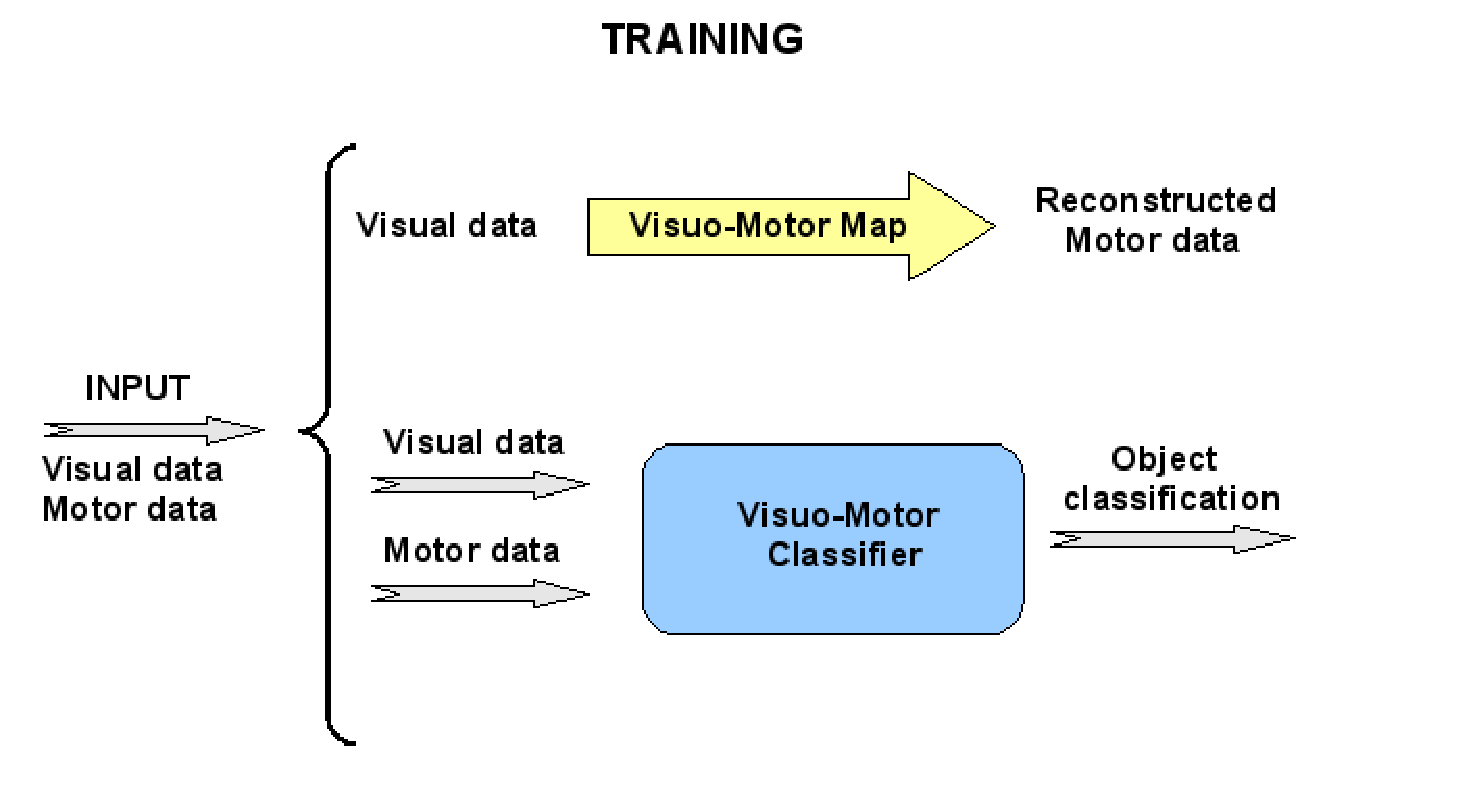
\includegraphics[width=0.48\textwidth]{images/train_fig_.pdf} &
    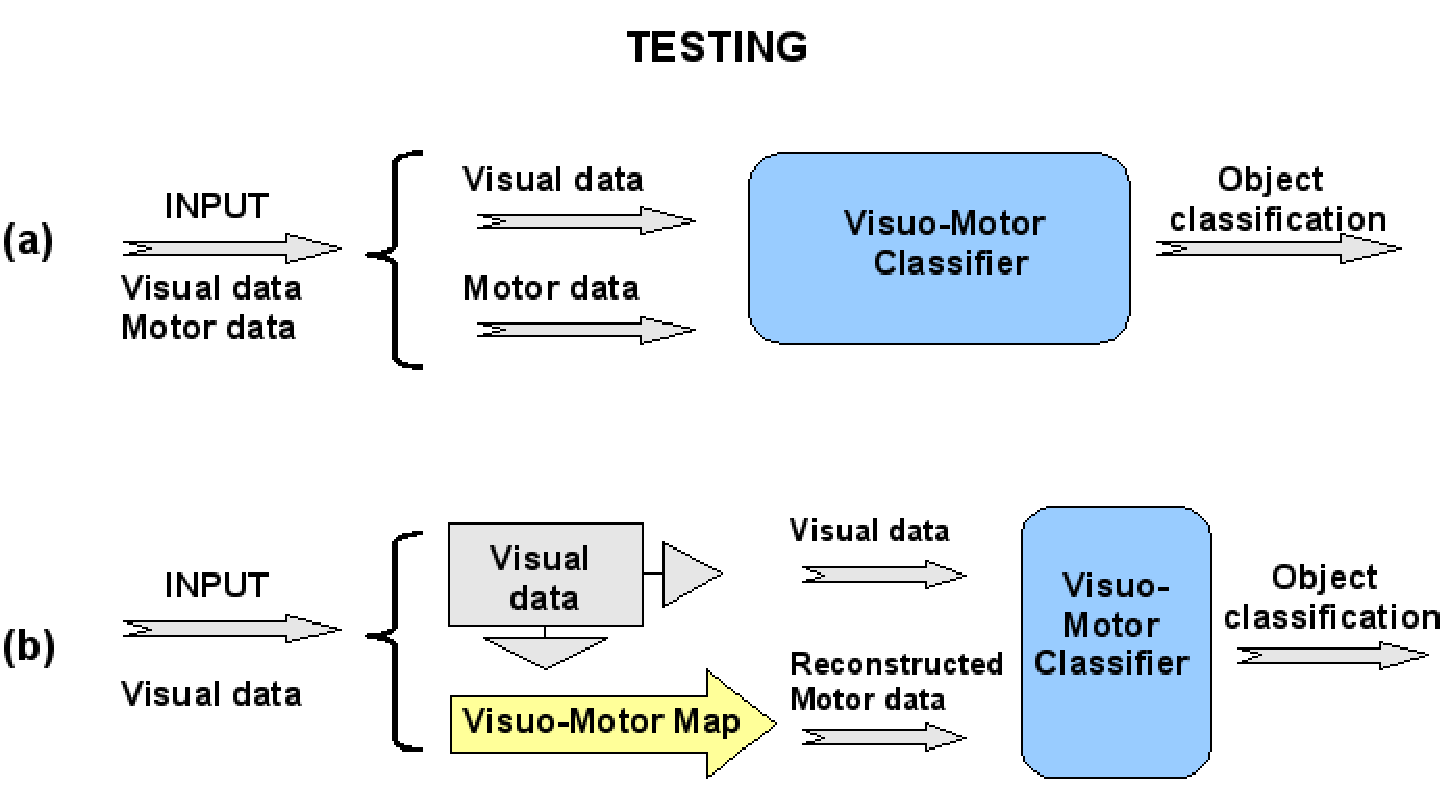
\includegraphics[width=0.48\textwidth]{images/test_fig_.pdf} \\
  \end{tabular}
  \caption{A schematic representation of the theoretical framework. During training (left), the system receives in input visual and
motor data, and it learns simultaneously a Visuo-Motor Map (VMM) and  Visuo-Motor Classifier (VMC). During testing (right), whenever
the agent sees but does not grasp the object, the VMM generates an archetypal grasp from the visual input, that is then used as
input to the multi modal classifier jointly with the perceived visual features.}
  \label{fig:framework}
\end{figure*}


%Willing to apply this idea to automated object recognition, we need to enrich
%an object model, traditionally consisting in a set of visual features,
%with motor features, obtained by reconstruction from the sight of the object.
%To carry on the biological analogy, we build a Visuo-Motor-Map (VMM) from human
%vision/grasping data to mimick the early-development training mentioned above.
%


%Schematically (consider Figure \ref{fig:training-scheme}), in a former phase we
%use visual \emph{and} motor data to build the VMM (\emph{sensorimotor map} in the general
%framework). In parallel, in order to check that motor information can actually be
%used to enrich traditional visual object classification, visual and motor features are
%fed to traditional classifier working upon visual features only, motor features
%only and both. We expect to see comparable performances obtained by each single-modal
%classifier, and a better performance obtained by the multi-modal classifier. (From now
%on we will denote the visual/motor features by VPR/MPR for Visual/Motor Perceptual
%Representation.)

%-scheme}. During training, the system receives as input labeled visual and motor
%perceptual representation. These correspond to the seen object (Visual Perceptual Representation, VPR) and to the grasp posture of the hand
%manipulating the object (Motor Perceptual Representation, MPR). On these data, the system builds in parallel two functions: a senso-motor map
%between VPR and MPR (Figure \ref{fig:test-scheme}, top) and a classification function receiving as input both modalities, trained
%to recognize the perceived object (Figure \ref{fig:training-scheme}, bottom). Technical details on how we compute the sensor motor map and the
%multi-modal classifier are reported in section \ref{sec::regression} and \ref{sec::classifier}


%Once the VMM has been built, and the hypothesis that multi-modal learning is better than
%single-modal has been verified, in a latter phase we test whether the VMM-reconstructed MPR
%can be used to the same extent the ``real'' MPR was. Figure \ref{fig:test-scheme} shows
%the test phase with its two possible outcomes. 
%
%
%  {\em Object classification}. Note that, having learned the object on two
%        modalities, the classifier needs as input a VPR and its corresponding MPR.
%        We derive the {\em not perceived} MPR using the senso-motor map (Figure
%        \ref{fig:test-scheme}, bottom) and give it as input to the classifier with
%        the VPR. We stress again that the clasifier recognizes the object on the
%        basis of its visual appearance and of how it can be grasped. Experiments
%        reported in section \ref{sec::experiments} shows clearly that this leads
%        to a significant increase in performance compared to using only visual
%        information.
%
